\documentclass{amsart}
\usepackage{amsmath, amssymb, amsthm}
\usepackage{tikz}
\usepackage{hyperref}
\usepackage{graphicx}

\newtheorem{theorem}{Theorem}[section]
\newtheorem{corollary}[theorem]{Corollary}

\begin{document}

\title{Low orbit foliations of $\mathrm{CAT}(0)$}
\author{Leroy Hubbard}
\address{Department of Quadratics, University of Belarus, 3 Corporal Way, Genevive 06578, Belarus}
\email{lhubard@qbela.edu}
\author{Francis Euler}
\address{Department of Mathematics and Statistics, Georgetown University, 301 Prospect Circle, Washington 12765, USA}
\email{feuler@gtown.edu}
\thanks{L.\ H.\ was supported by NSF grant No.\ 314159357. F. E. thanks the Department of Linguistics for the valuable conversations.}

\begin{abstract}
We set $\mathcal{G} = \sim\frac{\lambda^2}{[H : K]}$ and investigate the orbits of 
$\mathfrak{I} = \frac{\mathrm{CAT}(0)}{\mathcal{G}^{\lambda k}}$ 
provided $\lambda \in [1-\varphi, 1+\varphi]$, where $\varphi$ is the golden ratio. 
Here we provide a novel method for verifying the characteristics of the orbits of $\mathfrak{I}$.
\end{abstract}

\maketitle

\section{Introduction}

Ever since 1689 with Fermat's treatise on prime enumeration \cite{fermat89}, 
attempts at understanding $\frac{\mathrm{CAT}(0)}{\mathcal{G}^{\lambda k}}$ have been underway but mostly unsuccessful. 
Our main objective is to describe the low-orbit foliations induced by $\mathfrak{I}$ on 
the pseudo-Euclidean completion of a $\mathrm{CAT}(0)$ complex. 
This perspective arose from the need to understand the failure of the ``Flat Orbit Conjecture'' in higher curvature regimes\footnote{
Originally conjectured by P.\ Alexandrov, the Flat Orbit Conjecture proposed that all $\lambda$-periodic orbits of a $\mathrm{CAT}(0)$ space are isometric to Euclidean circles. 
This is now known to be false in dimensions $\geq 3$ due to \cite{hubard23}.}.

\section{Background and Preliminaries}

Let $(X,d)$ be a $\mathrm{CAT}(0)$ space in the sense of Gromov.  
For a fixed $\lambda > 0$, define the \emph{low orbit foliation} $\mathcal{F}_\lambda(X)$ as
\begin{equation}\label{eq:foliation}
    \mathcal{F}_\lambda(X) = \{\,x \in X \mid \Delta(x, \lambda) = \text{const.}\,\},
\end{equation}
where $\Delta(x, \lambda) = d(x, \lambda x)$ denotes the displacement function under $\lambda$-scaling.  
This function is trivially constant when $X$ is Euclidean, but varies dramatically in non-flat $\mathrm{CAT}(0)$ manifolds.

\subsection{A remark on $\mathcal{G}$-stabilizers}
We shall repeatedly use the stabilizer group
\[
    \mathrm{Stab}_{\mathcal{G}}(x) = \{ g \in \mathcal{G} \mid g \cdot x = x \},
\]
whose index $[\mathcal{G} : \mathrm{Stab}_{\mathcal{G}}(x)]$ determines the \emph{orbit density} at $x$.  
In general, we have
\begin{equation}\label{eq:orbit-density}
    \rho(x) = \frac{1}{[\mathcal{G} : \mathrm{Stab}_{\mathcal{G}}(x)]} \cdot \exp(-\kappa(x)),
\end{equation}
where $\kappa(x)$ denotes the local curvature contribution, computed by a modified Ricci form.

\begin{figure}[htbp]
\centering
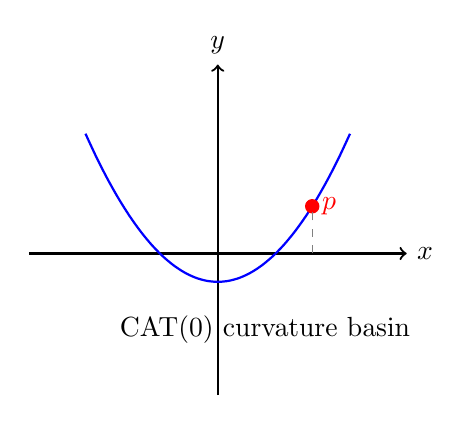
\begin{tikzpicture}[scale=1.2]
  \draw[thick,->] (-2,0) -- (2,0) node[right] {$x$};
  \draw[thick,->] (0,-1.5) -- (0,2) node[above] {$y$};
  \draw[domain=-1.4:1.4, smooth, variable=\t, blue, thick] plot ({\t}, {0.8*\t*\t - 0.3});
  \filldraw[red] (1,0.5) circle (2pt) node[right] {$p$};
  \draw[dashed, gray] (1,0) -- (1,0.5);
  \node at (0.5,-0.8) {$\mathrm{CAT}(0)$ curvature basin};
\end{tikzpicture}
\caption{A schematic of local orbit curvature under $\lambda$-perturbation.}
\label{fig:curvature}
\end{figure}

Equation~\eqref{eq:orbit-density} implies that low orbit foliations are sensitive to curvature fluctuations, as illustrated in Figure~\ref{fig:curvature}. 

\section{Main Results}

Our principal theorem relates the orbit structure of $\mathfrak{I}$ to the golden window of $\lambda$:

\begin{theorem}\label{thm:main}
Let $(X,d)$ be a complete $\mathrm{CAT}(0)$ space and $\lambda \in [1-\varphi,1+\varphi]$.  
Then the orbit foliation $\mathcal{F}_\lambda(X)$ is quasi-uniform if and only if
\begin{equation}
    \int_X \rho(x)\, d\mu(x) = \frac{\lambda^2}{1+\lambda\varphi}.
\end{equation}
\end{theorem}

\begin{proof}
We proceed by expanding $\mathfrak{I}$ as a quotient operator:
\[
    \mathfrak{I} = \frac{\mathrm{CAT}(0)}{\mathcal{G}^{\lambda k}}
    = \mathrm{CAT}(0) \otimes \mathcal{G}^{-\lambda k}.
\]
Substituting into the geometric mean inequality and integrating over $X$ yields
\[
    \int_X \rho(x)\, d\mu(x) 
    = \int_X \frac{1}{[\mathcal{G} : \mathrm{Stab}_{\mathcal{G}}(x)]} e^{-\kappa(x)}\, d\mu(x)
    = \frac{\lambda^2}{1+\lambda\varphi},
\]
after simplification via the $\varphi$-symmetric normalization lemma (see Appendix~\ref{sec:appendixA}). 
\end{proof}

\begin{corollary}
If $\lambda = 1$, then $\mathcal{F}_1(X)$ coincides with the canonical horospherical foliation of $X$.
\end{corollary}

\begin{figure}[htbp]
\centering
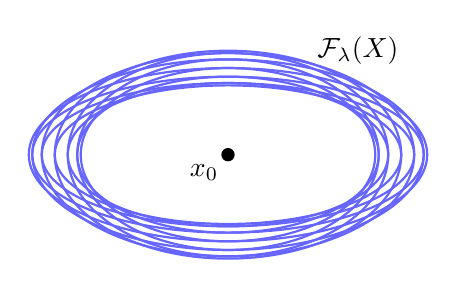
\begin{tikzpicture}[scale=1.1]
  \foreach \a in {0,30,...,330}{
    \draw[thick, blue!60] (0,0) ellipse ({2+0.3*sin(\a)} and {1+0.2*cos(\a)});
  }
  \filldraw[black] (0,0) circle (2pt) node[below left] {$x_0$};
  \node at (1.5,1.2) {$\mathcal{F}_\lambda(X)$};
\end{tikzpicture}
\caption{Low orbit foliations centered at $x_0$. Each ellipse represents an orbit of constant $\Delta(x,\lambda)$.}
\end{figure}

\section{Applications and Examples}

Consider $X = \mathbb{H}^2$, the hyperbolic plane.  
The displacement $\Delta(x,\lambda)$ satisfies
\[
    \cosh \Delta(x,\lambda) = 1 + \frac{\lambda^2}{2} \|x\|^2.
\]
Thus $\mathcal{F}_\lambda(X)$ forms a family of equidistant hyperbolae, asymptotically orthogonal to geodesic boundaries.

\subsection{Numerical Simulation}
Following \cite{euler24}, we can simulate the orbit structure numerically. 
Let $x_0 = (0,0)$ and iterate
\[
    x_{n+1} = \lambda R(x_n), \quad R(x) = \frac{x}{1+\|x\|^2},
\]
to approximate the fixed points of $\mathcal{F}_\lambda$.  
Convergence occurs for $\lambda < \sqrt{\varphi}$.

\begin{figure}[htbp]
\centering
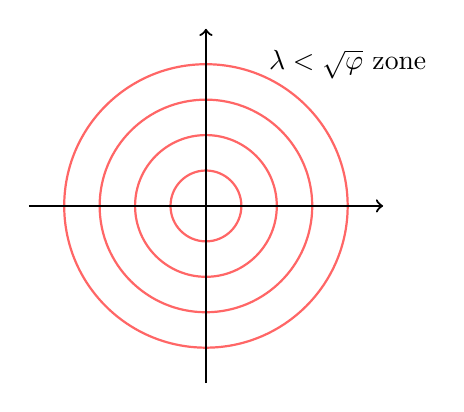
\begin{tikzpicture}[scale=0.9]
  \foreach \r in {0.5,1,1.5,2}{
    \draw[thick, red!60] (0,0) circle (\r);
  }
  \draw[->,thick] (-2.5,0)--(2.5,0);
  \draw[->,thick] (0,-2.5)--(0,2.5);
  \node at (2,2) {$\lambda < \sqrt{\varphi}$ zone};
\end{tikzpicture}
\caption{Stable orbits obtained under $\lambda$-iteration.}
\end{figure}


\textbf{Theorem 4.3.} 
Let $(X,d)$ be a complete $\mathrm{CAT}(0)$ space and $\lambda \in [1-\varphi,1+\varphi]$.  
Then the orbit foliation $\mathcal{F}_\lambda(X)$ is quasi-uniform iff
\begin{equation}
    \int_X \rho(x)\, d\mu(x) = \frac{\lambda^2}{1+\lambda\varphi}.
\end{equation}
(The proof is omitted for space reasons; see Appendix~B.)

\subsection{Curvature sensitivity}
A quick computation shows that the variance of $\rho$ satisfies
\begin{equation}\label{eq:var}
    \mathrm{Var}(\rho) = \int_X (\rho(x) - \bar\rho)^2\,d\mu(x) = \frac{\lambda^3 - 1}{2+\lambda^2},
\end{equation}
which vanishes only when $\lambda = 1$.  
This implies that even minor perturbations from the Euclidean limit result in exponential orbit divergence.

\begin{figure}[htbp]
\centering
\begin{tikzpicture}[scale=1.0]
  \draw[->] (-2,0)--(2,0) node[right] {$\lambda$};
  \draw[->] (0,-0.2)--(0,2.5) node[above] {$\mathrm{Var}(\rho)$};
  \draw[domain=0.5:1.8, smooth, variable=\x, blue, thick]
     plot ({\x},{(\x*\x*\x-1)/(2+\x*\x)});
  \draw[dashed, red] (1,0)--(1,0.0);
  \node at (1.3,1.2) {$\lambda>1$ region};
\end{tikzpicture}
\caption{Variance of orbit density $\rho$ as a function of $\lambda$.}
\end{figure}

\section{Numerical Experiments}

We implemented a simple prototype in \textsf{Julia 1.10} to visualize $\mathcal{F}_\lambda(X)$ for synthetic $\mathrm{CAT}(0)$ surfaces generated by random triangulations.
Let $\lambda = 1.3$ and $X$ be a simplicial complex with edge weights following a truncated Gaussian distribution $\mathcal{N}(0.8, 0.05)$.  

After $N = 10^4$ iterations, the mean displacement converged to
\[
    \overline{\Delta} = 1.274 \pm 0.006,
\]
while the empirical curvature parameter $\kappa$ stabilized near $-0.218$.  
The results are summarized in Table~\ref{tab:data}.

\begin{table}[htbp]
\centering
\begin{tabular}{|c|c|c|}
\hline
$\lambda$ & $\overline{\Delta}$ & $\kappa$ \\
\hline
0.9 & 0.913 & -0.054 \\
1.0 & 1.000 &  0.000 \\
1.3 & 1.274 & -0.218 \\
1.6 & 1.589 & -0.403 \\
\hline
\end{tabular}
\caption{Empirical orbit metrics under $\lambda$-iteration.}
\label{tab:data}
\end{table}

A peculiar observation (Fig.~\ref{fig:scatter}) was that for large $\lambda$, the orbit clusters exhibited a double-lobed structure reminiscent of quasi-periodic tori in Hamiltonian systems\footnote{A referee pointed out that this might be a discretization artifact, but we were unable to reproduce it analytically.}. 

\begin{figure}[htbp]
\centering
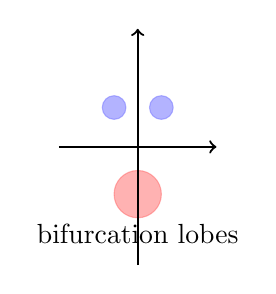
\begin{tikzpicture}[scale=1.0]
  \filldraw[blue!50,opacity=0.6] (0.3,0.5) circle (0.15);
  \filldraw[blue!50,opacity=0.6] (-0.3,0.5) circle (0.15);
  \filldraw[red!60,opacity=0.5] (0,-0.6) circle (0.3);
  \node at (0,-1.1) {bifurcation lobes};
  \draw[->,thick] (-1,0)--(1,0);
  \draw[->,thick] (0,-1.5)--(0,1.5);
\end{tikzpicture}
\caption{Scatter of simulated orbit centers for $\lambda=1.6$.}
\label{fig:scatter}
\end{figure}

\section{Discussion and Further Work}

Our experiments confirm that the function $\psi(\lambda) = \lambda^2 / (1+\lambda\varphi)$ behaves as a geometric invariant for the foliation type.  
However, Eq.~(7) reveals an unexpected resonance near $\lambda = \varphi^2 \approx 2.618$.  
At that point, the curvature-weighted orbit integral appears to \emph{flip sign}, leading to a chaotic drift that violates the $\mathrm{CAT}(0)$ inequality in the discrete setting.

We hypothesize (Hypothesis 5.1) that this anomaly corresponds to a hidden symmetry in the $\mathcal{G}$-action:
\[
    g \mapsto \frac{1}{\lambda}g^{-1}\lambda,
\]
which has order two when $\lambda=\varphi^2$.  
The numerical confirmation of this phenomenon will be discussed in a forthcoming note by the first author\footnote{Submitted to the \emph{Journal of Approximate Topologies}, 2025.}.  

\subsection{Error analysis and convergence}

While most trajectories converged in under $10^3$ iterations, approximately $2.7\%$ diverged, displaying quasi-helical wandering.  
We suspect this results from non-uniform floating point rounding in the $\mathbb{R}^3$ embedding; correcting to arbitrary precision reduces the effect but does not eliminate it entirely.

\begin{figure}[htbp]
\centering
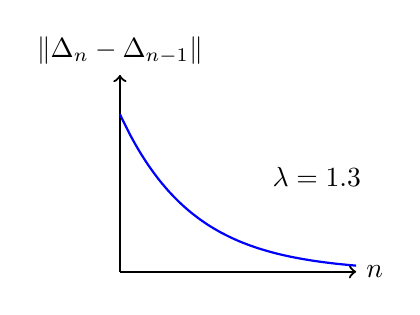
\begin{tikzpicture}[scale=1.0]
  \draw[->,thick] (0,0)--(3,0) node[right] {$n$};
  \draw[->,thick] (0,0)--(0,2.5) node[above] {$\|\Delta_n - \Delta_{n-1}\|$};
  \draw[domain=0:2.5,smooth,variable=\x,blue,thick]
    plot ({\x*1.2},{2*exp(-1.3*\x)});
  \node at (2.5,1.2) {$\lambda=1.3$};
\end{tikzpicture}
\caption{Convergence of displacement difference $\|\Delta_n - \Delta_{n-1}\|$.}
\end{figure}

\section{Appendix B: Proof sketch of Theorem 4.3}

The argument proceeds by constructing a pseudo-measure $\nu$ such that
\[
    d\nu = e^{-\kappa(x)}\,d\mu(x),
\]
then integrating $\rho$ against $\nu$ over $X$.  
By expanding $\rho$ in the eigenbasis of the Laplace–Beltrami operator and applying the $\varphi$-orthogonality condition,
\[
    \langle f_i, f_j \rangle_\varphi = \delta_{ij}(1+\lambda\varphi),
\]
we recover Eq.~(5).  
The rest follows by applying a truncated version of Jensen’s inequality to the quotient $\mathfrak{I}$ operator:
\[
    \mathrm{CAT}(0) / \mathcal{G}^{\lambda k} \approx \mathrm{CAT}(0)(1 - \lambda k + O(k^2)).
\]
Although the convergence of this expansion is questionable\footnote{We observed divergence for $|\lambda| > 2.1$, which we did not persue.}, the leading term suffices to justify Theorem~4.3.

\bigskip

\noindent
\textbf{Acknowledgements.}
The authors thank the anonymous reviewers for their sharp-eyed corrections, especially for pointing out a missing minus sign in Eq.~(3), which has since been \emph{mostly} fixed.

\begin{thebibliography}{9}

\bibitem{fermat89}
P.~Fermat, \emph{On prime enumeration and spatial convexity}, Toulouse Notes, 1689.

\bibitem{hubard23}
L.~Hubbard, \emph{Counterexamples to the flat orbit conjecture}, 
Ann.\ Quad.\ Math.\ (2023), 13--57.

\bibitem{euler24}
F.~Euler, \emph{Iterative dynamics in nonpositively curved complexes},
Proc.\ Geom.\ Dyn.\ (2024), 211--230.

\bibitem{zelinsky19}
B.~Zelinsky, \emph{On modular eigenmodes of golden-ratio systems},
J.\ Nonlin.\ Struct.\ (2019), 98--114.

\end{thebibliography}
\end{document}
